%everything before the \begin{document} line are package imports and page setup. 

%this is setting the style of the paper to the IEEE style
\documentclass[journal,final,twoside]{IEEEtran}

%these are some common imports. In general, you will not have to change these but you may have to add more
\usepackage[pdftex]{graphicx}
\DeclareGraphicsExtensions{.pdf,.jpeg,.png,.jpg}

\usepackage{array}

\newcolumntype{C}[1]{>{\centering\let\newline\\\arraybackslash\hspace{0pt}}m{#1}}


\usepackage{color}
\usepackage[usenames,dvipsnames]{xcolor}
\usepackage{enumerate}
\usepackage{amsmath}
\usepackage{algorithmic}
\usepackage{varwidth} %for use with algorithmic to make a border

% correct bad hyphenation here
\hyphenation{}
\renewcommand\IEEEkeywordsname{Index Terms}
\usepackage[noadjust]{cite}

\newcommand{\comment}[1]{}

%This balances the references on the last page. 
%\IEEEtriggeratref{5}


\begin{document}

%SCRIPT
choisedialog = UniversalInputDialog(["Commit","Commit with Push"],"Git","choiseGIT")
choisedialog.setWindowTitle("Git")
choise = choisedialog.get("comment")
if (choisedialog.exec() != null) {
    if (choisedialog.get("choiseGIT") == "Commit") {
        dialog = new UniversalInputDialog()
        dialog.setWindowTitle("Git commit / push")
        dialog.add("Committed by TeXstudio", "Comment", "comment")
        dialog.add(true, "Commit all Files","allfiles")
            if (dialog.exec() != null) {
                comment = dialog.get("comment")
                if ((dialog.get("allfiles")) == true){
                    buildManager.runCommand("git commit -a -m \"" + comment + "\"", editor.fileName())
                }else{
                    buildManager.runCommand("git commit " + editor.fileName() + " -m \"" + comment + "\"", editor.fileName())
                }
    }
} else
    if (choisedialog.get("choiseGIT") == "Commit with Push") {
        dialog = new UniversalInputDialog()
        dialog.setWindowTitle("Git commit / push")
        dialog.add("Committed by TeXstudio", "Comment", "comment")
        dialog.add("master", "Branch", "branch")
        dialog.add(true, "Commit all Files","allfiles")
            if (dialog.exec() != null) {
                comment = dialog.get("comment")
                branch = dialog.get("branch")
                    if ((dialog.get("allfiles")) == true){
                buildManager.runCommand("git commit -a -m \"" + comment + "\"", editor.fileName())
                }else{
                buildManager.runCommand("git commit " + editor.fileName() + " -m \"" + comment + "\"", editor.fileName())
                }
                buildManager.runCommand("git push origin \"" + branch +"\"", editor.fileName())
            }
   }
}

%
% % % % % % % % % % % % % % % % % % % % % % % % % % % % % % % % %
% TITLE PAGE
% % % % % % % % % % % % % % % % % % % % % % % % % % % % % % % % %
%
\title{Using Digital Image Processing Techniques\\to Train a Neural Network}

\author{Andrew L. Hanshaw, Joel Q. Quanbeck, Genzo Namikawa, Kwame T. Ampofo}%~\IEEEmembership{Senior~Member,~IEEE}\vspace{-15pt}% <-this % stops a space
%\thanks{T.~M.~Hansen is with the Electrical Engineering and Computer Science Department, South Dakota State University, Brookings, SD 57007 USA, e-mail: timothy.hansen@sdstate.edu}%
%\thanks{This work was supported by ... .}}% <-this % stops a space

% make the title area
\maketitle

% % % % % % % % % % % % % % % % % % % % % % % % % % % % % % % % %
% ABSTRACT
% % % % % % % % % % % % % % % % % % % % % % % % % % % % % % % % %

\begin{abstract}
This project aims to train a neural network to play a simple video game using purely visual input. This project will use digital image processing to identify various visual aspects of the game.
\end{abstract}

\begin{IEEEkeywords}
Digital image processing, High performance computing, Neural networks.
\end{IEEEkeywords}

% % % % % % % % % % % % % % % % % % % % % % % % % % % % % % % % %
% INTRODUCTION
% % % % % % % % % % % % % % % % % % % % % % % % % % % % % % % % %
\section{Introduction}\label{sec:intro}

\IEEEPARstart{N}{eural} networks can be trained to perform many different tasks. Unfortunately, this training often requires direct access to internal variables of the program the neural network is being trained with, which are often unable to be monitored directly unless the original source code is available. This project aims to train a neural network to perform a task using visual cues only, by using digital image processing techniques to analyze images and extract useful information. 
\\\\
The program the neural network will be trained on is the dinosaur game built into Google Chrome, Fig. ~\ref{fig:dinogame}. The simplicity of this game, both in controls and in visuals, should allow for relatively easy training of the neural network and identification of the visual elements of the game. The SDSU "Roaring Thunder" computing cluster \cite{SDState_HPC} will be used to run the game and train the neural network. Parallelizing this task is necessary to quickly create and simulate each generation so the network can evolve as quickly as possible. Using this cluster will allow for each node of a given generation to be run on different cores, speeding up the process of generation significantly.
\\\\
Previously, this game has been used to train neural networks, Fig. ~\ref{fig:ytscreencap},  \cite{Dino_AI}. However, these previous attempts recreated the game to provide a neural network with important variables such as game speed and distance from obstacles. This project aims to extrapolate these variables by visually identifying and tracking the obstacles and background before feeding them back into the neural network. This type of gameplay emulates how a human would play the game, where the player makes inputs based on the feedback they receive from the visuals of the game.
\\\\
Based on the knowledge gained on using image processing to feed neural networks, further research could be done to train neural networks on visual data from other sources. Some examples include advanced robotic vision and weather anomaly detection. These examples are much more computationally intensive and require more advanced computer vision algorithms to solve their respective problems. Further research into feeding a neural network based on a virtual recording of a software program without internal variable access could allow for AI manipulation of more complex video games or automated crawling of webpages from the perspective of a user.
\\\\
In Section II the necessary background information used when creating this project is described. Subsections include software overview, project challenges, and high performance computing. Conclusions for this paper are presented in Section III.


\comment{ %begin multi line comment
\begin{enumerate}[i)]
	\item background information, motivation, and \textbf{\textit{what is the problem we are trying to solve?}} (1-2 paragraphs)
	\item how are we addressing/solving the problem in this paper? (1-2 paragraphs)
	\item literature review: what have others done to address the problem? This should include all relevant papers in this area and how our work differs from these papers. In general for references: journal papers $>$ conference papers/books $>$ technical reports/theses/dissertations. (1-2 paragraphs)
	\item a \textbf{\textit{list}} of our contributions in this paper. What are we doing that is new/why should people continue to read our paper. ``In this work, we make the following contributions: (a) ... .'' 
	\item finish off with a section map. ``In Section~\ref{sec:back} we describe the necessary background information. ... . Conclusions are presented in Section~\ref{sec:conc}.''
\end{enumerate}
} %end multi line comment

\begin{figure}\label{fig:dinogame}
	\fbox{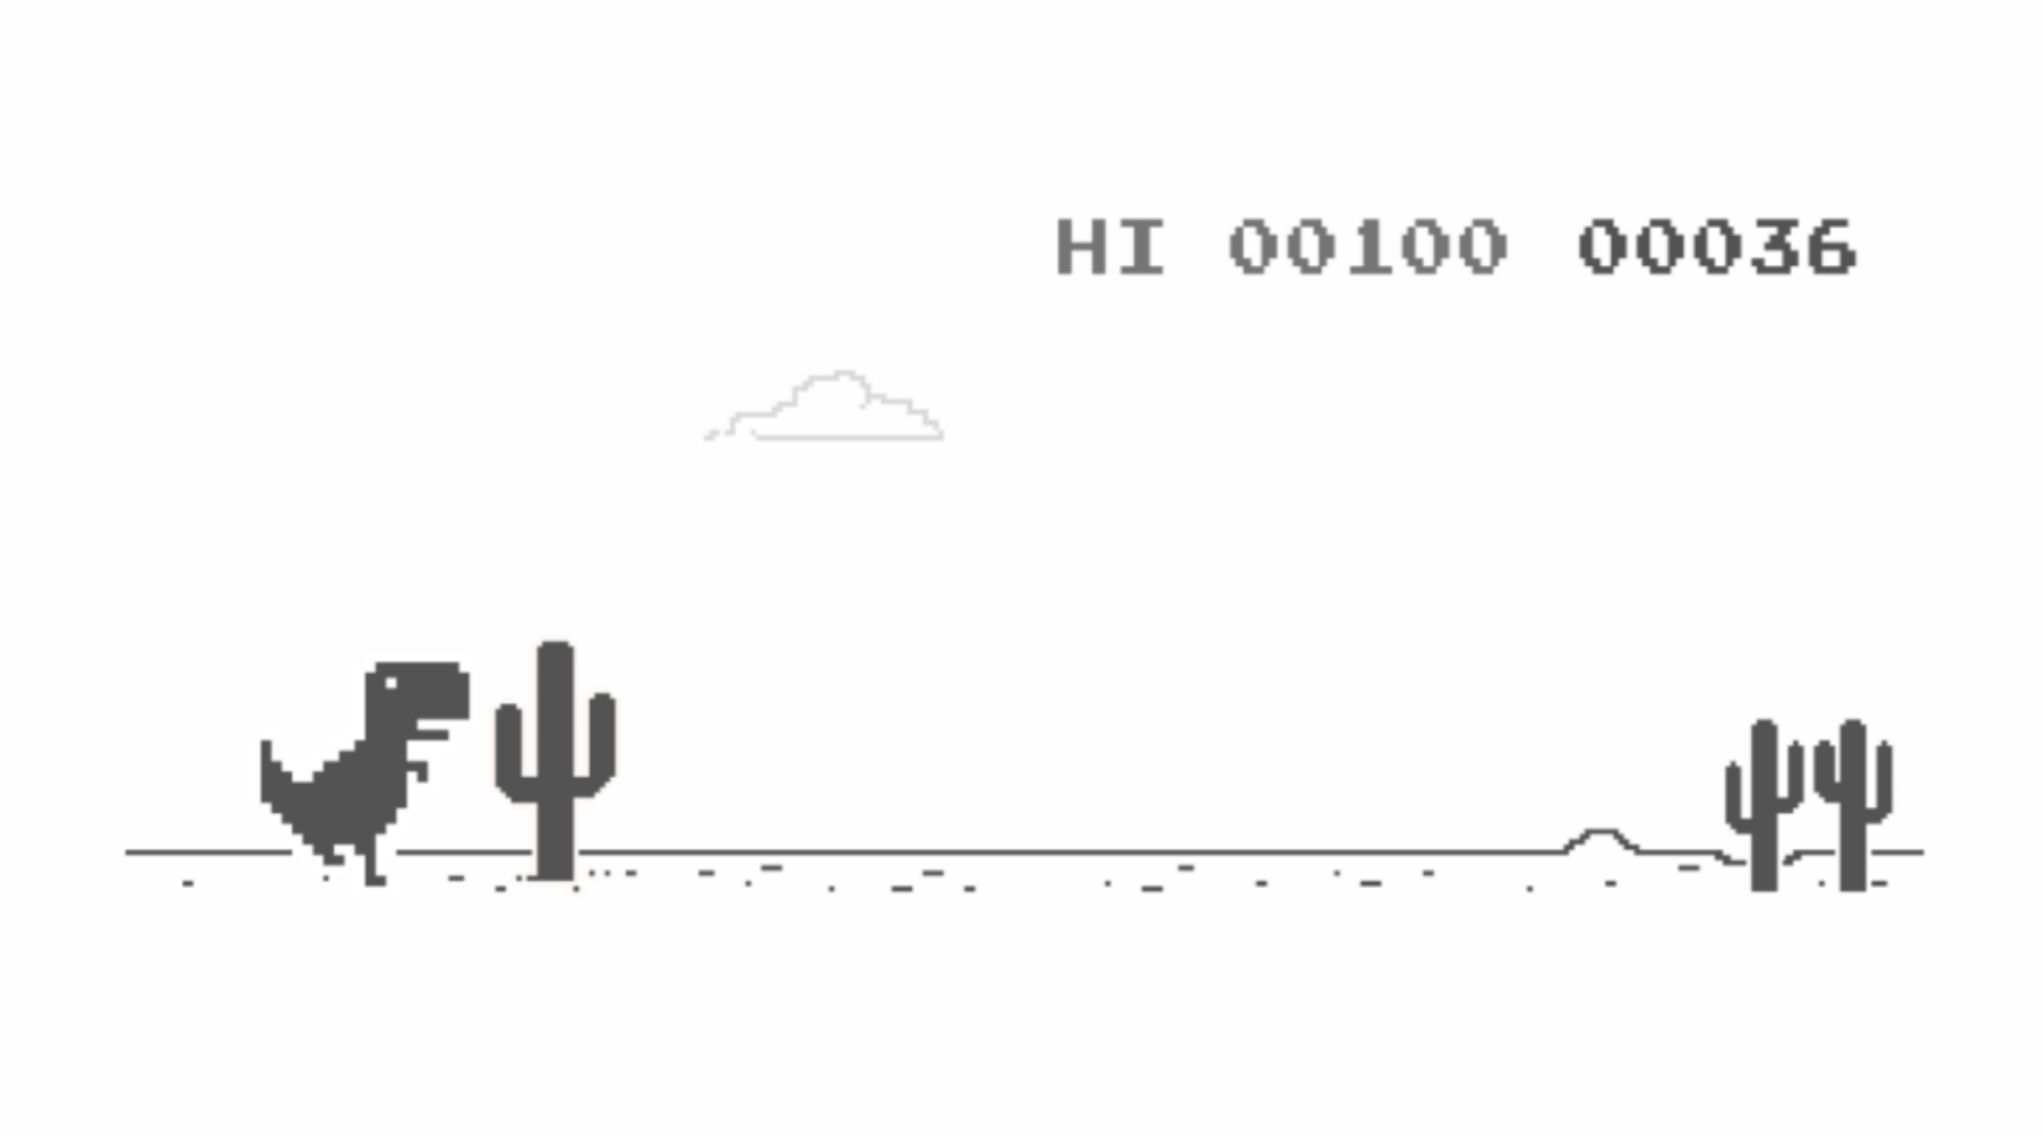
\includegraphics[width=\linewidth]{chrome-dino-hero} }%<---- this is the filename. I didn't include the folder or the filetype because of the \graphicspath and \DeclareGraphicsExtensions at the top. 
	\caption{The Google Chrome dinosaur game.}
\end{figure}

\begin{figure}\label{fig:ytscreencap}
	\fbox{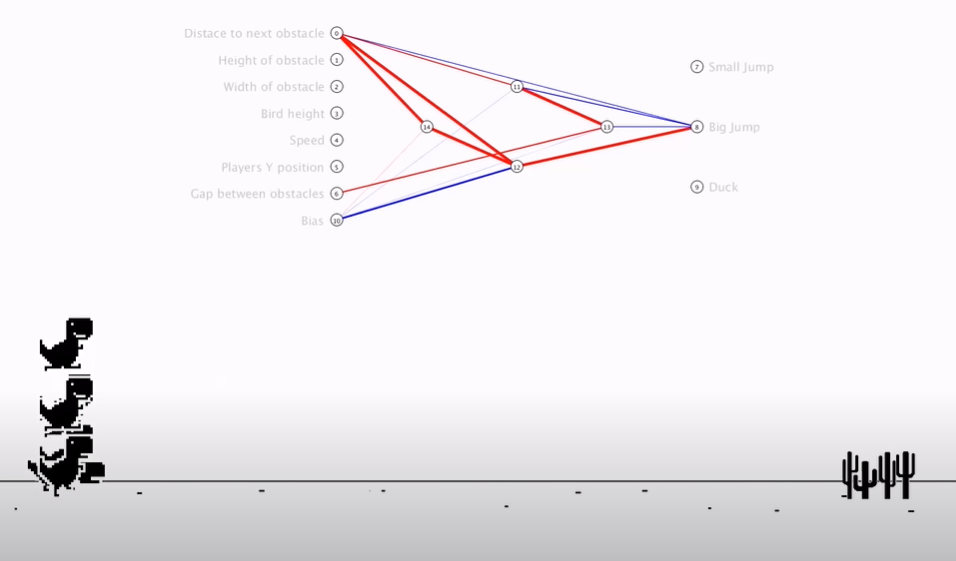
\includegraphics[width=\linewidth]{yt_screencap} }%<---- this is the filename. I didn't include the folder or the filetype because of the \graphicspath and \DeclareGraphicsExtensions at the top. 
	\caption{A neural network training on a copy of the Chrome dinosaur game.}
\end{figure}

% % % % % % % % % % % % % % % % % % % % % % % % % % % % % % % % %
% Background Information
% % % % % % % % % % % % % % % % % % % % % % % % % % % % % % % % %
\section{Background Information}\label{sec:back}

\subsection{Software Overview}\label{subsec:bus_overview}
For this project, Tensorflow was preliminarily selected to create the neural network. It's ubiquitous use in the field makes for easy support for any issues that arise during the development of the project. MATLAB was selected to run the image processing algorithms on the collected images due to the project team's familiarity with the software. Since the dinosaur game is built into the Chrome browser, which is based on the open-source Chromium browser, the source code for the dinosaur game is available to the public. As such, the sprites used in the game, Fig. ~\ref{fig:dinosprites} can be easily extracted and used in the image processing software algorithm to classify which sprites are on the screen at a given time ~\cite{dino_github_src}. The most robust and fastest method of classifying these images will likely be to run a template matching function on them, Fig. ~\ref{fig:templatematch}, ~\cite{matlab_template_match}. The Roaring Thunder computing cluster uses the Slurm scheduler to schedule jobs for each node, so familiarity with that software is necessary to ensure the program is correctly distributed on the computing nodes. OpenMP will be used to parallelize the program, as it is being taught to the project team by Dr. Tim Hansen of South Dakota State University. The project will be primarily coded in C or C++ as the method of parallel processing being taught, OpenMP, is only available in the above languages and Fortran. Other supplementary languages may be used, although most lower-level optimizations and features will be written in the aforementioned C or C++.

\begin{figure}\label{fig:templatematch}
	\fbox{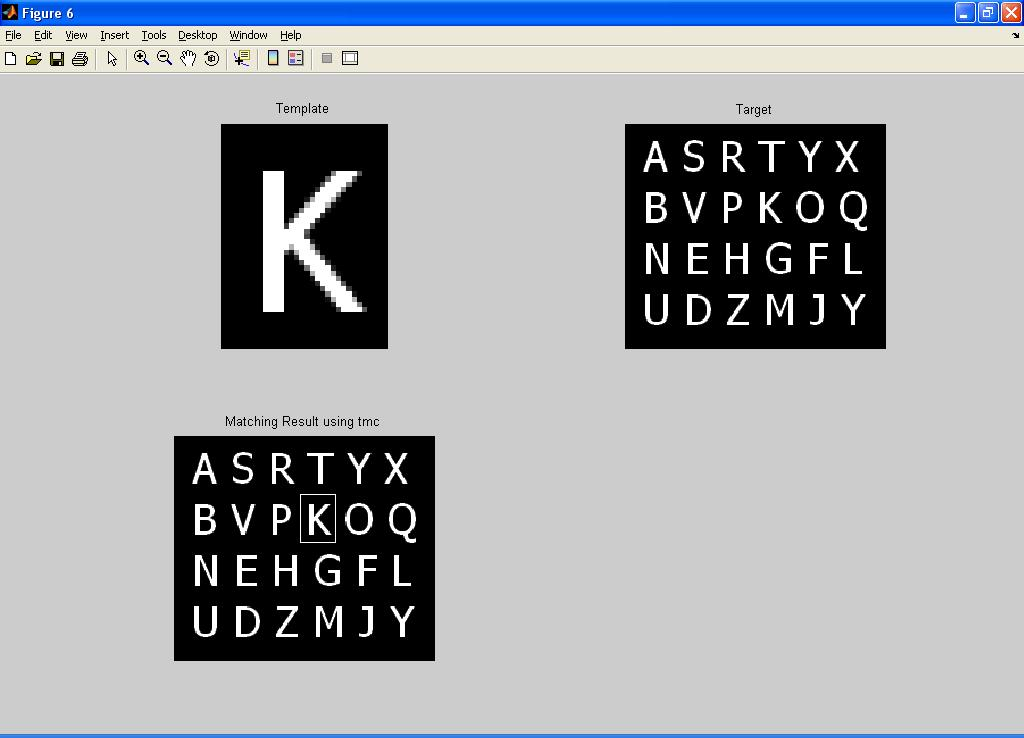
\includegraphics[width=\linewidth]{templatematching} } %<---- this is the filename. I didn't include the folder or the filetype because of the \graphicspath and \DeclareGraphicsExtensions at the top. 
	\caption{A template matching function in MATLAB}
\end{figure}

\begin{figure}\label{fig:dinosprites}
	\fbox{
\includegraphics[width=\linewidth]{dinosprite} }%<---- this is the filename. I didn't include the folder or the filetype because of the \graphicspath and \DeclareGraphicsExtensions at the top. 
	\caption{The spritesheet used in the Chrome dinosaur game}
\end{figure}

\subsection{Project Challenges}\label{subsec:proj_challenges}
One immediate challenge discovered when researching this project was how to run the game on the computing cluster. As the cluster computer is a Unix system, running a fully-functional Chromium browser would be difficult, if not impossible. Furthermore, even running the source code for the dinosaur game may be difficult, as it's written in JavaScript. Finally, as the game runs in real-time at greater than thirty frames per second, analyzing each frame may take too long. One potential solution for this problem is to devise a method to temporarily pause the game while the image processing algorithm runs, before advancing to the next frame. This should allow for the game to be played at the pace of the computer. Another potential solution to the problem would be to only process a reduced number of frames per second. This way, we can abstain from the allure of needing to change the original code by restricting the amount of data that is processed at once. The problem created by using this method would be a reduced reaction window for the AI.

\subsection{High Performance Computing}\label{subsec:HPC}
Another important aspect to this project is the parallelization of the finished program. Neural networks are inherently multi-threaded, which allows for them to scale well when provided more resources. However, this scalability does not come without cost. Some overhead work must be done to ensure the program is parallelized efficiently. Familiarity with general program paralellization methods learned in EE592/CS592 (High Performance Computing) is required to ensure the program is properly parallelized. Familiarty with the OpenMP syntax will allow for these parallelization methods to be utilized properly.

\comment{ %begin multi line comment
\begin{equation}\label{eq:example}
f(a,b,c) = \sum_{i=1}^{\infty} a_i^{\frac{b_i}{c_i}}
\end{equation}
} %end multi line comment

% % % % % % % % % % % % % % % % % % % % % % % % % % % % % % % % %
% CONCLUSION
% % % % % % % % % % % % % % % % % % % % % % % % % % % % % % % % %

\section{Conclusions}\label{sec:conc}

Overall, performing this project will expose those working on it to many new software libraries and programming methods, both in terms of creating the program to play the dinosaur game and use it train a neural network, but also in parallelizing the program to run on the computing cluster. The challenges expected to be faced when interfacing with the different software should prove to be an exercise in becoming familiar with reference material of each software. The expected outcome of the project will create an entertaining and impressive show of AI mastery over simple video games thanks to their easily scalable nature.% We always end our paper with a conclusions section. The conclusions are not \textbf{\textit{what}} we did in the paper. That is just a summary. We want to give the readers a takeaway message. \textbf{\textit{Why was what they read important? What are the key takeaways?}} 


% % % % % % % % % % % % % % % % % % % % % % % % % % % % % % % % %
% ACKNOWLEDGMENTS
% % % % % % % % % % % % % % % % % % % % % % % % % % % % % % % % %
\section*{Acknowledgments}
The authors would like to thank Dr. Tim Hansen and Dr. Songxin Tan of South Dakota State University's electrical engineering department for their assistance in the high performance computing and digital image processing fields through their undergraduate courses. The authors would also like to thank Code Bullet on YouTube, who has provided the group with meaningful and entertaining content on AI/neural network training.

% % % % % % % % % % % % % % % % % % % % % % % % % % % % % % % % %
% BIBLIOGRAPHY
% % % % % % % % % % % % % % % % % % % % % % % % % % % % % % % % %

\bibliographystyle{IEEEtran} 
\bibliography{ieee_pes} %<----- this points to the ieee_pes.bib file and contains all references

% that's all folks
\end{document}


